\documentclass[aspectratio=169]{beamer}
   \usetheme{metropolis}
   \setbeamertemplate{blocks}[rounded][shadow=false]
\usepackage{url}
\usepackage{hyperref}
\usepackage{booktabs}
\usepackage{tabularx}
\usepackage{dcolumn}
   \newcolumntype{d}[1]{D{.}{.}{#1}}
\usepackage{graphicx}
\usepackage[justification=raggedright]{caption}
\usepackage{adjustbox}
\usepackage{color}
\usepackage{textpos}
\usepackage{etoolbox}
\usepackage[cache=true,cachedir=minted_cache]{minted}
\usepackage{multimedia}
\usepackage [english]{babel}
\usepackage [autostyle, english = american]{csquotes}
\MakeOuterQuote{"}

\captionsetup[figure]{justification=centering}

\makeatletter
\patchcmd{\beamer@sectionintoc}{\vskip1.5em}{\vskip0.5em}{}{}
\makeatother

\definecolor{smured}{rgb}{0.797,0,0.027}
\definecolor{smublue}{RGB}{48,64,116}
\definecolor{dkgreen}{rgb}{0,0.6,0}
\definecolor{gray}{rgb}{0.5,0.5,0.5}
\definecolor{mauve}{rgb}{0.58,0,0.82}
\definecolor{text_gray}{RGB}{46,58,62}

\setbeamercolor{progress bar}{fg=smured,bg=smublue}
\setbeamercolor{title separator}{fg=smublue}
\setbeamercolor{frametitle}{bg=smublue}
\setbeamersize{description width=16pt}

\metroset{
  numbering=fraction
}

\hypersetup{
  colorlinks=true,
  allcolors=text_gray,
  urlcolor=smured,
}

\addtobeamertemplate{frametitle}{}{
\begin{textblock*}{1cm}(\textwidth,-1.155cm)

\includegraphics[width=1cm]{figures/smu_logo.pdf}
\end{textblock*}}

\setminted{breaklines,linenos,fontsize=\scriptsize}
\setmintedinline{fontsize=auto}

\title{MPI, NCCL, and NVSHMEM}
\author{John LaGrone\\ HPC Applications Scientist}
\institute{
Research and Data Sciences Services\\
Office of Information Technology\\
Center for Research Computing\\
Southern Methodist University}
\date{February 23, 2022}

\begin{document}

\begin{frame}
\titlepage
\end{frame}

\begin{frame}{Outline}
\footnotesize
\tableofcontents[hideallsubsections]
\end{frame}

\section{Research Support}

\begin{frame}{Research and Data Science Services}
\begin{table}
\small
\begin{tabularx}{\textwidth}{Xll}
\toprule
Domain & Name & Email \\
\midrule
Data Science & Dr.\ Eric Godat & \href{mailto:egodat@smu.edu}{egodat@smu.edu} \\
High-Performance Computing & Dr.\ Robert Kalescky & \href{mailto:rkalescky@smu.edu}{rkalescky@smu.edu} \\
& Dr.\ John LaGrone & \href{mailto:jlagrone@smu.edu}{jlagrone@smu.edu} \\
Machine Learning \& Artificial Intelligence & Dr.\ Tue Vu & \href{mailto:tuev@smu.edu}{tuev@smu.edu} \\
Custom Devices (IOT, wearables, etc.) & Guillermo Vasquez & \href{mailto:guillermov@smu.edu}{guillermov@smu.edu} \\
Human Trafficking Data Analyst & Mateo Langston-Smith & \href{mailto:mlangstonsmith@smu.edu}{mlangstonsmith@smu.edu} \\
\bottomrule
\end{tabularx}
\caption{The OIT Research and Data Science Services team provides research computing support, consultations, and collaborations.}
\end{table}
\end{frame}

\begin{frame}{Data Science Institute (DSI)}
\begin{itemize}
  \item Maintains our primary shared resource for research computing in collaboration with OIT
  \item Provides research computing tools, support, and training to all faculty, staff, and students using research computing resources
  \item \url{https://southernmethodistuniversity.github.io/hpc_docs/} has documentation and news
  \item \href{mailto:help@smu.edu}{help@smu.edu} or \href{mailto:rkalescky@smu.edu}{rkalescky@smu.edu} or \href{mailto:jlagrone@smu.edu}{jlagrone@smu.edu} for help
  \item Request an account at \url{https://southernmethodistuniversity.github.io/hpc_docs/}
\end{itemize}
\end{frame}


\section{Message Passing Interface (MPI)}

\begin{frame}{Motivation}
\begin{itemize}
\item MPI is a specification of what the interface should look like and what it should do
\begin{itemize}
\item Separate processes on each node communicate by sending and receiving data over a network
\item MPI can be used for parallelism on a single node as well
\end{itemize}
\item An MPI implementation is a set of libraries that allow for multiple nodes to be used together via message passing
\item Many higher-level languages and libraries support or use MPI
\item MPI has become the industry standard for distributed-memory programming
\end{itemize}
\end{frame}

\begin{frame}{MPI Implementations}
\begin{itemize}
\item Open source
\begin{itemize}
\item MPICH
\item OpenMPI
\item MVAPICH
\end{itemize}
\item Closed source
\begin{itemize}
\item Intel MPI (based on MPICH)
\item Mellanox HPC-X MPI (based on OpenMPI)
\end{itemize}
\end{itemize}
\end{frame}

\begin{frame}{Compiling MPI Programs}
Depending on your programming language and the specific MPI implementation,
these wrapper scripts can have different names
\begin{itemize}
\item C++: mpicxx or mpic++
\item C: mpicc
\item Fortran 90/95/2003: mpif90
\item Fortran 77: mpif77
\end{itemize}
\end{frame}

\begin{frame}{Running MPI Programs}
\begin{itemize}
\item Running MPI batch jobs on ManeFrame is almost identical to running serial
      and OpenMP batch jobs. However, when running MPI jobs, we must tell the
      queueing system a few additional pieces of information:
\begin{enumerate}
\item How many total nodes we want to reserve on the machine?
\item How many total cores do we want to reserve on the machine?
\item How do you want to distribute tasks on each node?
\item How many MPI tasks do you actually want to run?
\end{enumerate}
\item We have two key ways to control execution of parallel batch jobs:
\begin{itemize}
\item Controlling how the job is reserved
\item Controlling how the MPI job is executed
\end{itemize}
\end{itemize}
\end{frame}

\subsection{Examples}
\subsubsection{Estimating \(\pi\)}

\begin{frame}{Estimating \(\pi\)}
\begin{listing}[H]
\inputminted[firstline=1, lastline=7]{C}{examples/mpi/mpi_monte_carlo_pi.c}
\caption{Includes and function prototypes}
\end{listing}
\end{frame}

\begin{frame}{Estimating \(\pi\)}
\begin{listing}[H]
\inputminted[firstline=35, lastline=48]{C}{examples/mpi/mpi_monte_carlo_pi.c}
\caption{Function definitions.}
\end{listing}
\end{frame}

\begin{frame}{Estimating \(\pi\)}
\begin{listing}[H]
\inputminted[firstline=9, lastline=15]{C}{examples/mpi/mpi_monte_carlo_pi.c}
\caption{Argument check and variable initialization.}
\end{listing}
\end{frame}

\begin{frame}{Estimating \(\pi\)}
\begin{listing}[H]
\inputminted[firstline=16, lastline=21]{C}{examples/mpi/mpi_monte_carlo_pi.c}
\caption{Initialize MPI, get the global number of tasks, and get the process rank.}
\end{listing}
\end{frame}

\begin{frame}{Estimating \(\pi\)}
\begin{listing}[H]
\inputminted[firstline=22, lastline=27]{C}{examples/mpi/mpi_monte_carlo_pi.c}
\caption{Get number of hits per rank via summation reduction.}
\end{listing}
\end{frame}

\begin{frame}{Estimating \(\pi\)}
\begin{listing}[H]
\inputminted[firstline=28, lastline=33]{C}{examples/mpi/mpi_monte_carlo_pi.c}
\caption{If rank zero, report estimation of \(\pi\). All ranks finalize and exit.}
\end{listing}
\end{frame}

\begin{frame}{Estimating \(\pi\)}
\begin{listing}[H]
\inputminted[firstline=6, lastline=8]{Bash}{examples/mpi/README.md}
\caption{Build executable.}
\end{listing}
\end{frame}

\begin{frame}{Estimating \(\pi\)}
\begin{listing}[H]
\inputminted[firstline=1, lastline=8]{Bash}{examples/mpi/mpi_monte_carlo_pi.sbatch}
\caption{Reguest compute resources.}
\end{listing}
\end{frame}

\begin{frame}{Estimating \(\pi\)}
\begin{listing}[H]
\inputminted[firstline=10]{Bash}{examples/mpi/mpi_monte_carlo_pi.sbatch}
\caption{Setup environment and run.}
\end{listing}
\end{frame}


\section{MPI for Python}

\begin{frame}{Installing  \mintinline{sh}{mpi4py}}
\begin{description}
\item  \mintinline{sh}{mpi4py} should be installed with \mintinline{sh}{pip} when possible
\item \mintinline{sh}{Conda} installed versions will likely be built with an unoptimized version of MPI
\item There can be significant performance impacts, especially for communication bound applications
\end{description}
\end{frame}

\begin{frame}[fragile]{\mintinline{sh}{Conda} \mintinline{sh}{mpi4py} Demo}
	Minimal example of  \mintinline{sh}{mpi4py} using \mintinline{sh}{Conda}
\begin{minted}{sh}
	# load version of Python that has Conda in it
	module load python/3
	
	# create a virtual environment named conda_mpi4py that uses Python 3.9 
	# and installs mpi4py
	conda create -p $HOME/conda_mpi4py mpi4py python=3.9 
\end{minted}
\end{frame}

\begin{frame}[fragile]{\mintinline{sh}{pip} \mintinline{sh}{mpi4py} Demo}
	Minimal example of  \mintinline{sh}{mpi4py} using \mintinline{sh}{pip}
	\begin{minted}{sh}
		# load Intel compilers, which include a version of Python and an MPI compiler
		module load intel
		
		# create a virtual environment named venv_mpi4py
		python -m venv ~/venv_mpi4py
		
		# upgrade pip
		pip install --upgrade pip
		
		# make sure we're using the correct MPI compiler
		export MPICC=$(which mpicc)
		
		# install mpi4py, the flags --no-binary :all: --compile 
		# tell pip not to use a precompiled version
		pip install --no-binary :all: --compile mpi4py
	\end{minted}
\end{frame}

\begin{frame}[fragile]{Bandwidth Test}
	We'll use a simple bandwidth test available here \url{https://github.com/felker/mpi4py_benchmark}
	
\textbf{Important commands:}
	
	Import the \mintinline{sh}{mpi4py} libraries
	\begin{minted}{python}
		from mpi4py import MPI
	\end{minted}

    Creating a communicator and getting ranks:
    \begin{minted}{python}
    	comm = MPI.COMM_WORLD
    	myid = comm.Get_rank()
    	numprocs = comm.Get_size()
    \end{minted}
\end{frame}

\begin{frame}[fragile]{Bandwidth Test}
	
	Create send and receive buffers
	\begin{minted}{python}
		# create the message. [data_buffer size type]
		if (id == 0):
			s_msg = [s_buf, size, MPI.BYTE]
			r_msg = [r_buf,    4, MPI.BYTE]
		elif (if == 1):
		 	s_msg = [s_buf, 4, MPI.BYTE]
		 	r_msg = [r_buf,    size, MPI.BYTE]
	\end{minted}
	
	Send and receive requests
	\begin{minted}{python}
		if (id == 0):
			requests = comm.Isend(s_msg, 1, 100)
			MPI.Request.Waitall(requests)
			comm.Recv(r_msg, 1, 101)
		elif (id == 1):
			requests = comm.Irecv(r_msg, 0, 100)
			MPI.Request.Waitall(requests)
			comm.Send(s_msg, 0, 101)
	\end{minted}
\end{frame}

\begin{frame}[fragile]{Running with \mintinline{sh}{Conda} \mintinline{sh}{mpi4py}}
	\inputminted{sh}{examples/mpi4py/run_conda_env.sbatch}
\end{frame}

\begin{frame}[fragile]{Running with \mintinline{sh}{venv} \mintinline{sh}{mpi4py}}
	\inputminted{sh}{examples/mpi4py/run_venv.sbatch}
\end{frame}

\begin{frame}[fragile]{Example Output}
	\inputminted{text}{examples/mpi4py/sample_output.txt}
\end{frame}


\section{NVIDIA Collective Communications Library (NCCL)}

\begin{frame}{NCCL}
\begin{itemize}
\item NCCL is a communication library designed primarily for inter-GPU communications
\item It is not (currently) a stand alone parallel programming framework 
\item Generally, NCCL uses is very similar to MPI
\end{itemize}
\end{frame}

\begin{frame}{Why Do We Need NCCL?}
	\begin{figure}
		\centering
		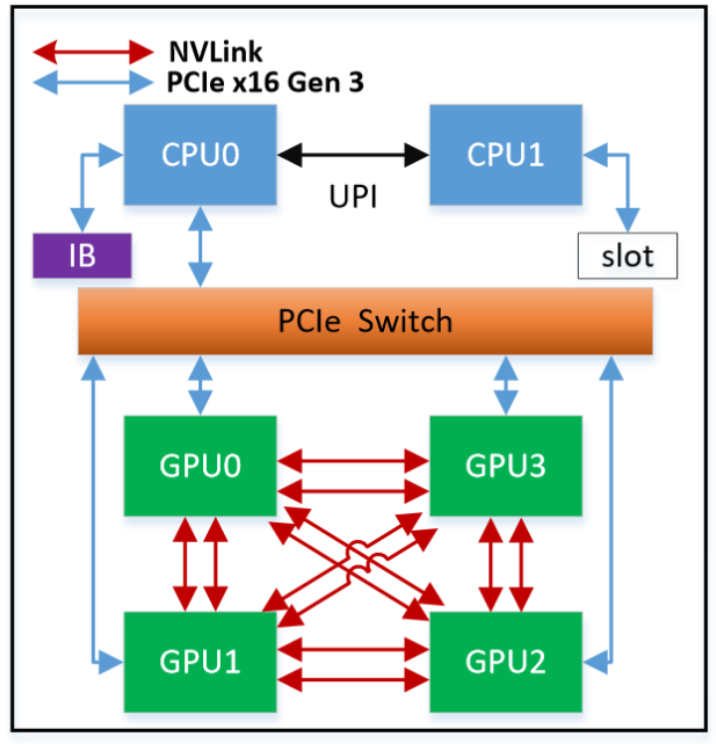
\includegraphics[width=0.45\linewidth]{figures/example_gpu_node_interconnect.png}
		\caption{An example of a possible multi-GPU node configuration}
	\end{figure}
\end{frame}

\begin{frame}[fragile]{NCCL Collective Operations}

\begin{minted}{c}
	// AllReduce
	ncclResult_t ncclAllReduce(const void* sendbuff, void* recvbuff, size_t count, ncclDataType_t datatype, ncclRedOp_t op, ncclComm_t comm, cudaStream_t stream)
	
	// Broadcast
	ncclResult_t ncclBroadcast(const void* sendbuff, void* recvbuff, size_t count, ncclDataType_t datatype, int root, ncclComm_t comm, cudaStream_t stream)
	
	// Reduce
	ncclResult_t ncclReduce(const void* sendbuff, void* recvbuff, size_t count, ncclDataType_t datatype, ncclRedOp_t op, int root, ncclComm_t comm, cudaStream_t stream)
	
	// AllGather
	ncclResult_t ncclAllGather(const void* sendbuff, void* recvbuff, size_t sendcount, ncclDataType_t datatype, ncclComm_t comm, cudaStream_t stream)
	
	// ReduceScatter
	ncclResult_t ncclReduceScatter(const void* sendbuff, void* recvbuff, size_t recvcount, ncclDataType_t datatype, ncclRedOp_t op, ncclComm_t comm, cudaStream_t stream)
\end{minted}
\end{frame}

\begin{frame}[fragile]{NCCL Point to Point Operations}
	
	Note, these are non-blocking.
	
	\begin{minted}{c}
		// Send
		ncclResult_t ncclSend(const void* sendbuff, size_t count, ncclDataType_t datatype, int peer, ncclComm_t comm, cudaStream_t stream)
		
		// Receive
		ncclResult_t ncclRecv(void* recvbuff, size_t count, ncclDataType_t datatype, int peer, ncclComm_t comm, cudaStream_t stream)
	\end{minted}
\end{frame}

\begin{frame}[fragile]{General Flow}
	
	\begin{minted}{c}
		// initialize MPI
		int myRank, nRanks, localRank = 0;
		MPI_Init(&argc, &argv);
		MPI_Comm_rank(MPI_COMM_WORLD, &myRank);
		MPI_Comm_size(MPI_COMM_WORLD, &nRanks);
		
		// initialize NCCL
		int nDev = 4;
		int devs[4] = { 0, 1, 2, 3 };
		ncclComm_t comms[4];
		ncclCommInitAll(comms, nDev, devs);
	\end{minted}
\end{frame}

\begin{frame}[fragile]{General Flow}
	
	\begin{minted}{c}
		// allocate and initializing device buffers
		float** sendbuff = (float**)malloc(nDev * sizeof(float*));
		float** recvbuff = (float**)malloc(nDev * sizeof(float*));
		cudaStream_t* s = (cudaStream_t*)malloc(sizeof(cudaStream_t)*nDev);
		
		
		for (int i = 0; i < nDev; ++i) {
			cudaSetDevice(i);
			cudaMalloc(sendbuff + i, size * sizeof(float));
			cudaMalloc(recvbuff + i, size * sizeof(float));
			cudaMemset(sendbuff[i], 1, size * sizeof(float));
			cudaMemset(recvbuff[i], 0, size * sizeof(float));
			cudaStreamCreate(s+i);
		}
	
	\end{minted}
\end{frame}

\begin{frame}[fragile]{General Flow}
	
	\begin{minted}{c}
		// Do some NCCL communication. Group API is required when using
		// multiple devices per thread
		ncclGroupStart();
		for (int i = 0; i < nDev; ++i)
		 	ncclAllReduce((const void*)sendbuff[i], (void*)recvbuff[i], size, ncclFloat, ncclSum,	comms[i], s[i]);
		ncclGroupEnd();
		
		
		// Make sure operations are synchronized by waiting for stream to finish
		for (int i = 0; i < nDev; ++i) {
			cudaSetDevice(i);
			cudaStreamSynchronize(s[i]);
		}
	\end{minted}
\end{frame}

\begin{frame}[fragile]{General Flow}
	
	\begin{minted}{c}
		// free device buffers
		for (int i = 0; i < nDev; ++i) {
			cudaSetDevice(i);
			cudaFree(sendbuff[i]);
			cudaFree(recvbuff[i]);
		}
		
		
		// finalizing NCCL
		for(int i = 0; i < nDev; ++i)
			ncclCommDestroy(comms[i]);
			
		// finalize MPI
		MPI_Finalize()
	\end{minted}
\end{frame}

\begin{frame}[fragile]{Example on M2}
	
	Run a simple benchmark on M2 from \url{https://github.com/NVIDIA/nccl-tests}
	
	\begin{minted}{sh}
		# get repository
		git clone git@github.com:NVIDIA/nccl-tests.git
		
		# change directory to the repository
		cd nccl-tests
		
		# load NVHPC module
		module load nvhpc-21.9
		
		# build with MPI enabled
		make MPI=1 CUDA_HOME=/hpc/applications/nvidia/hpc_sdk/2021_21.9/Linux_x86_64/21.9/cuda/11.4/
	\end{minted}
\end{frame}

\begin{frame}[fragile]{Run on 4 P100 nodes }
	\inputminted[fontsize=\tiny]{sh}{examples/nccl/p100x4.sbatch}
\end{frame}

\begin{frame}[fragile]{Run on 4 P100 nodes }
	\inputminted[fontsize=\tiny]{sh}{examples/nccl/p100x4.txt}
\end{frame}

\begin{frame}[fragile]{Run on 2 V100s on 2 nodes }
	\inputminted{sh}{examples/nccl/v100_2x2.sbatch}
\end{frame}

\begin{frame}[fragile]{Run on 2 V100s on 2 nodes}
	\inputminted[fontsize=\tiny]{sh}{examples/nccl/v100_2x2.txt}
\end{frame}

\begin{frame}[fragile]{Run on 4 V100s on 1 node }
	\inputminted{sh}{examples/nccl/v100_4x1.sbatch}
\end{frame}

\begin{frame}[fragile]{Run on 4 V100s on 1 node}
	\inputminted[fontsize=\tiny]{sh}{examples/nccl/v100_4x1.txt}
\end{frame}


\section{NVSHMEM}

\begin{frame}{Motivation for NVSHMEM}
\begin{itemize}
\item Programming model for efficient and scalable multi-GPU codes.
\item Based on OpenSHMEM.
\item Provides a partitioned global address space (PGAS) that spans the memory
      of all included GPUs.
\item Communication is initiated directly from the GPUs, which can be more
      performant than CPU-bound distributed programming models.
\end{itemize}
\end{frame}

\subsection{Examples}
\subsubsection{Estimating \(\pi\)}

\begin{frame}{Estimating \(\pi\)}
\begin{listing}[H]
\inputminted[firstline=1, lastline=14]{C++}{examples/nvshmem/nvshmem_pi.cpp}
\caption{Includes and definitions.}
\end{listing}
\end{frame}

\begin{frame}{Estimating \(\pi\)}
\begin{listing}[H]
\inputminted[firstline=16, lastline=32]{C++}{examples/nvshmem/nvshmem_pi.cpp}
\caption{Monte Carlo method for estimating \(\pi\) CUDA kernel.}
\end{listing}
\end{frame}

\begin{frame}{Estimating \(\pi\)}
\begin{listing}[H]
\inputminted[firstline=35, lastline=45]{C++}{examples/nvshmem/nvshmem_pi.cpp}
\caption{Initialize NVSHMEM and get local processing element (PE) ID and global number of PEs.}
\end{listing}
\end{frame}

\begin{frame}{Estimating \(\pi\)}
\begin{listing}[H]
\inputminted[firstline=47, lastline=53]{C++}{examples/nvshmem/nvshmem_pi.cpp}
\caption{Allocate memory on hosts and devices and initialize the number of hits.}
\end{listing}
\end{frame}

\begin{frame}{Estimating \(\pi\)}
\begin{listing}[H]
\inputminted[firstline=55, lastline=65]{C++}{examples/nvshmem/nvshmem_pi.cpp}
\caption{Launch kernel on the devices to perform the computations, block until
all are finished, and then accumulate the results.}
\end{listing}
\end{frame}

\begin{frame}{Estimating \(\pi\)}
\begin{listing}[H]
\inputminted[firstline=67, lastline=77]{C++}{examples/nvshmem/nvshmem_pi.cpp}
\caption{Only on the first PE, copy accumlated hits back to host and report estimated value of \(\pi\).}
\end{listing}
\end{frame}

\begin{frame}{Estimating \(\pi\)}
\begin{listing}[H]
\inputminted[firstline=79, lastline=87]{C++}{examples/nvshmem/nvshmem_pi.cpp}
\caption{Free memory on hosts and device, finalize NVSHMEM, and exit.}
\end{listing}
\end{frame}

\begin{frame}{Estimating \(\pi\)}
\begin{listing}[H]
\inputminted[firstline=1, lastline=8]{Bash}{examples/nvshmem/nvshmem_pi.sbatch}
\caption{Reguest compute resources.}
\end{listing}
\end{frame}

\begin{frame}{Estimating \(\pi\)}
\begin{listing}[H]
\inputminted[firstline=10, lastline=16]{sh}{examples/nvshmem/nvshmem_pi.sbatch}
\caption{Setup the environment. \mintinline{sh}{$GCC_HOME} is to provide full C++ 11 support.}
\end{listing}
\end{frame}

\begin{frame}{Estimating \(\pi\)}
\begin{listing}[H]
\inputminted[firstline=18, lastline=25]{sh}{examples/nvshmem/nvshmem_pi.sbatch}
\caption{Build the executable for the specific PE being used and run.}
\end{listing}
\end{frame}


\begin{frame}{Help?}
\centering
Need help or have questions?\\
\href{mailto:rkalescky@smu.edu}{rkalescky@smu.edu} \\
\href{mailto:jlagrone@smu.edu}{jlagrone@smu.edu} \\
\href{mailto:help@smu.edu}{help@smu.edu}  (include HPC in the subject line)
\end{frame}



\end{document}

